\begin{scanpage}{0049}{32}
\begin{center}\begin{minipage}[t]{.48\linewidth}\vspace{0pt}\centering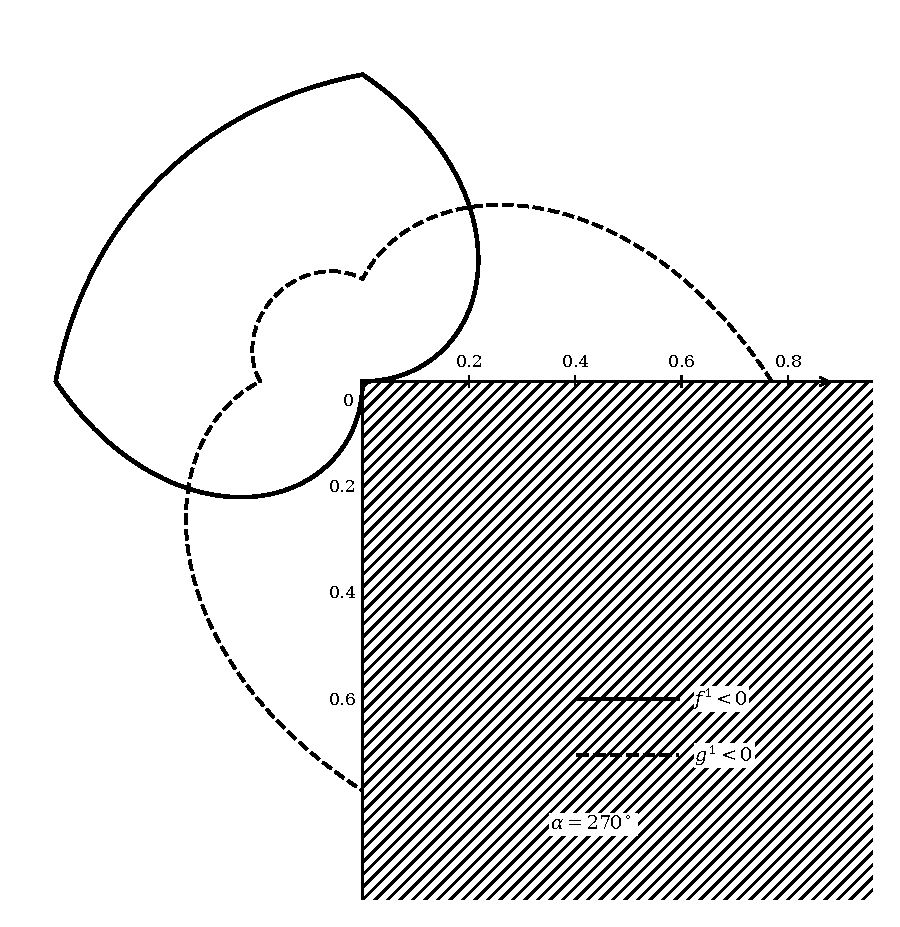
\includegraphics[height=7cm,width=.98\linewidth,keepaspectratio]{images/recreated/a-0049-fig12.pdf}\par Figure 12. The same as Figure 10 for the case $\phi=\phi_0$.\end{minipage}\hfill\begin{minipage}[t]{.48\linewidth}\vspace{0pt}\centering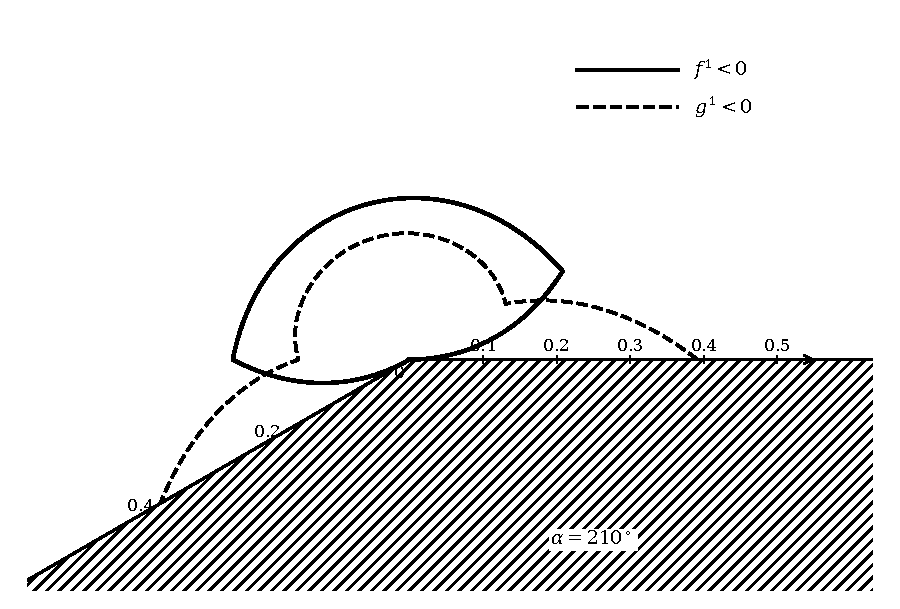
\includegraphics[height=5cm,width=.98\linewidth,keepaspectratio]{images/recreated/a-0049-fig13.pdf}\par Figure 13. The functions $f^1$ and $g^1$ for a wedge $(\phi=\phi_0,\ \alpha=210^\circ)$.\end{minipage}\end{center}
the field scattered by composite bodies, we will not integrate the explicit expressions for the nonuniform part of the current, but we will endeavour to express these integrals directly in terms of the functions $f^1$ and $g^1$ which have been found.
\sectiontitle{5}{The Oblique Incidence of a Plane Wave on a Wedge}
Above, the diffraction was studied of a plane wave incident on a wedge perpendicular to its edge. Now let us investigate the case when the plane wave
\[\mathbf E=\mathbf E_0e^{ik(x\cos\alpha+y\cos\beta+z\cos\gamma)}\tag{5.01}\]
falls on the wedge at an oblique angle $\gamma$ $\left(0<\gamma<\frac\pi2\right)$ to the wedge edge (Figure 14).

From the geometry of the problem, it follows that the diffraction field must have that same dependence on the $z$ coordinate as the field of the incident wave, that is
\end{scanpage}
